\documentclass[11pt]{article}

\usepackage{amsmath, amssymb, bm, graphicx}

% Margins
\topmargin=-0.45in
\evensidemargin=0in
\oddsidemargin=0in
\textwidth=6.5in
\textheight=9.0in
\headsep=0.25in

\title{DSPotential Theory Document}
\author{ David Moeller Sztajnbok }
\date{March, 2024}

\begin{document}
\maketitle

%--Paper--

\section{Brief Vector Calculus Review}
Before diving into the differential equations that govern fluid flow, particularly the flow we are interested in - irrotational, incompressible flow - a brief review of vector calculus is useful for the math that is to follow. This document will be void of complicated derivations, but will still include basic vector calculus concepts and notation. Below is a brief review of these concepts. \\
\subsection{Vector Notation}
This document will use standardized notation throughout, some of which is presented below.\\ \\
\noindent
Vectors are denoted by an arrow above them and are also bolded. A velocity vector, for instance, is denoted $\vec{\bm{u}}$ while a scalar quantity, density, is denoted $\rho$.\\ \\
\noindent
Vectors are presented in matrix form to more easily visualize operations like dot products, cross products, and vector multiplication. They are presented as an $nx1$ matrix, that is, a column vector. The example of velocity vector is shown below:

\begin{equation*}
    \vec{\bm{u}} = \begin{bmatrix}
                    u \\
                    v \\
                    w \\
                    \end{bmatrix}
\end{equation*}

\noindent
Where $u, v, $ and $w$ are the $x, y, $ and $z$ components of vector $\vec{\bm{u}}$. \\

\subsection{Vector Operations}
It is important to remember the different vector operations. Addition and subtraction are ommited from the discussion below. The focus is given to the scalar, vectorial, and simple multiplication of vectors, also known as the dot, cross, and simple products. 
\subsubsection{The Dot Product}
Consider two vectors $\vec{\bm{a}}$ and $\vec{\bm{b}}$ such that:

\begin{equation*}
    \vec{\bm{a}} = \begin{bmatrix}
        a_x \\
        a_y \\
        a_z \\
    \end{bmatrix}
\end{equation*}

And

\begin{equation*}
    \vec{\bm{b}} = \begin{bmatrix}
        b_x \\
        b_y \\
        b_z \\
    \end{bmatrix}
\end{equation*}

\noindent
Then the dot product between them is:

\begin{equation*}
    \vec{\bm{a}} \cdot \vec{\bm{b}} = a_xb_x + a_yb_y + a_zb_z
\end{equation*}

\noindent
With the geometric meaning that the dot product is the magnitude of the projection of $\vec{\bm{a}}$ onto $\vec{\bm{b}}$, also given by:

\begin{equation*}
    \vec{\bm{a}} \cdot \vec{\bm{b}} = \lvert\vec{\bm{a}}\rvert \lvert\vec{\bm{b}}\rvert\cos{\theta}
\end{equation*}

\noindent
Where $\theta$ is the angle formed between $\vec{\bm{a}}$ and $\vec{\bm{b}}$.\\ \\ \\
\noindent
\emph{Note: the dot product is an operation between two vectors and it results in a scalar. It is not to be confused with the multiplication of a scalar by a vector:}
\begin{equation*}
    c\vec{\bm{a}} = \begin{bmatrix}
        ca_x \\
        ca_y \\
        ca_z \\
    \end{bmatrix}
\end{equation*}
\emph{Where $c$ is a constant. The operation above is the product between a scalar and a vector, and results in a vector! So be weary of the dots in the text below.}

\subsubsection{The Cross Product}
Consider the same vectors as before. The cross product between them is:

\begin{equation*}
    \vec{\bm{a}} \times \vec{\bm{b}} = \begin{vmatrix}
        \hat{i} & \hat{j} & \hat{k} \\
        a_x & a_y & a_z \\
        b_x & b_y & b_z
    \end{vmatrix} = \hat{i}\begin{vmatrix}
        a_y&a_z\\b_y&b_z
    \end{vmatrix} - \hat{j}\begin{vmatrix}
        a_x&a_z\\b_x&b_z
    \end{vmatrix} + \hat{k}\begin{vmatrix}
        a_x&a_y\\b_x&b_y
    \end{vmatrix} = \hat{i}(a_yb_z - a_zb_y) + \hat{j}(a_zb_x-a_xb_z) + \hat{k}(a_xb_y - a_yb_x)
\end{equation*}\\

\noindent
With the geometric meaning that the cross product is a vector normal to both $\vec{\bm{a}}$ and $\vec{\bm{b}}$ and its magnitude is the area formed by the parallellepiped between $\vec{\bm{a}}$ and $\vec{\bm{b}}$. This magnitude is:

\begin{equation*}
    \vec{\bm{a}} \times \vec{\bm{b}} = \lvert\vec{\bm{a}}\rvert \lvert\vec{\bm{b}}\rvert\sin{\theta}
\end{equation*}\\

\noindent
Where $\theta$ is the angle between the vectors. Note that the cross product is an operation between two vectors that yields another vector.

\subsection{Scalar vs. Vector Fields}
It is important to make a subtle yet important distinction before speaking of derivatives. In fluid flow, we are interested in calculating different properties at different points in space and time. Therefore, quantities will be functions of space ($x, y, \textnormal{and}\ z$) and time ($t$.) \emph{However, these quantities can be scalar and/or vectors.}\\\\
\noindent
A vector field is a function of space and time wherein each point in space and time defines a vector. The best example and perhaps the most relevant here is the velocity vector, $\vec{\bm{u}}$:

\begin{equation*}
    \vec{\bm{u}} = u\hat{i} + v\hat{j} + w\hat{k}
\end{equation*}\\
\noindent
Wherein each component of the velocity is a function of space and time:


\begin{eqnarray*}
    u = u(x, y, z, t)\\
    v = v(x, y, z, t)\\
    w = w(x, y, z, t)
\end{eqnarray*}\\
\noindent
Therefore at each point in space at a given time, each component of the velocity vector at that point in space and time is defined, and a vector is therefore defined at that point.\\ \\
\noindent
Scalar fields, on the other hand, are scalars defined as functions of space and time. Thus, instead of a point in space and time defining three components that form a vector, only a scalar is defined. The best examples are pressure and temperature:
\begin{eqnarray*}
    P = P(x, y, z, t)\\
    T = T(x, y, z, t)\\
\end{eqnarray*}

\subsection{The Gradient of a Scalar Field}
Consider a scalar field $p(x,y,z)$. It defines a pressure (scalar) at every point in space. We are often interested in the direction at which the pressure increases the most, and the rate at which it increases. This is given by the gradient of the scalar field, $\nabla p$. \\ \\
\noindent
The gradient of a scalar field $\nabla p$ is defined as the vector with the following properties:
\begin{enumerate}
    \item Its direction is towards the greatest increase in the scalar field and;
    \item Its magnitude is the rate of increase of the scalar field in that direction.
\end{enumerate}
\noindent
The gradient vector, $\nabla$ is defined as:
\begin{equation*}
    \nabla = \begin{bmatrix}
                \frac{\partial}{\partial x} \\
                \frac{\partial}{\partial y} \\
                \frac{\partial}{\partial z} \\     
                \end{bmatrix}
\end{equation*}
\noindent
Such that the gradient of the scalar field is simply:
\begin{equation*}
    \nabla p = \begin{bmatrix}
                \frac{\partial p}{\partial x} \\
                \frac{\partial p}{\partial y} \\
                \frac{\partial p}{\partial z} \\     
                \end{bmatrix}
\end{equation*}

\subsection{Curl and Divergence}
\noindent
Another important set of concepts important in vector calculus that involve the gradient operator, $\nabla$, are the curl and divergence of a vector field. The curl of a vector field $\vec{\bm{A}}$ is given by:

\begin{equation*}
    \textnormal{curl}(\vec{\bm{A}}) = \nabla \times \vec{\bm{A}}
\end{equation*}

\noindent
While the divergence of a vector field $\vec{\bm{A}}$ is given by:

\begin{equation*}
    \textnormal{div}(\vec{\bm{A}}) = \nabla \cdot \vec{\bm{A}}
\end{equation*} \\ 
\noindent
Note that both the curl and divergence operations are performed on vectors. However, the curl produces a vector while the divergence produces a scalar.\\ \\ 
\noindent
This will show itself useful when we define the concepts of rotationality, as well as the fundamental condition for the conservation of mass. \\

\subsection{Total Derivative}
\noindent
In single-variable calculus, functions are dependent on one variable only. Therefore, some function $f(x)$ has as its derivative $\frac{df}{dx}$ and will be a function of x and x only (or some constant.)\\ \\
\noindent
In multivariable calculus, however, functions are dependent on more than one variable. It is typically the case in fluid flow that quantities are functions of space ($x, y,$ and $z$) as well as time ($t$) which can be typically written as $f(x, y, z, t)$. However, the one of the variables in the function can be itself a function of another variable. It is imperative in that case to make use of the chain rule when differentiating the function, just as was the case in single-variable calculus when differentiating compound functions. \\ \\
\noindent
Let us consider a practical example. The acceleration of a fluid particle is given by:

\begin{equation*}
    \vec{\bm{a}} = \frac{d}{dt}[\vec{\bm{u}}(\vec{\bm{r}}, t)]
\end{equation*}

\noindent
Where $\vec{\bm{r}}$ is the position vector given by:

\begin{equation*}
    \vec{\bm{r}} = \begin{bmatrix}
                    r_x \\
                    r_y \\
                    r_z \\     
                    \end{bmatrix}
\end{equation*}

\noindent
And the components of the velocity vector $\vec{\bm{u}}$ are given by:

\begin{equation*}
    \vec{\bm{u}} = \begin{bmatrix}
                    u \\
                    v \\
                    w \\     
                    \end{bmatrix}
\end{equation*}

\noindent
The total derivative $\frac{d}{dt}[\vec{\bm{u}}(\vec{\bm{r}}, t)]$ must account for changes in position as functions of time, as well as changes in the velocity components as functions of position and time. The chain rule must be applied The total derivative is from now on denoted $\frac{D}{Dt}$ and is given by:

\begin{equation*}
    \frac{D\vec{\bm{u}}}{Dt} = \frac{\partial\vec{\bm{u}}}{\partial t} + \frac{\partial\vec{\bm{u}}}{\partial x}\frac{\partial x}{\partial t} + \frac{\partial\vec{\bm{u}}}{\partial y}\frac{\partial y}{\partial t} + \frac{\partial\vec{\bm{u}}}{\partial z}\frac{\partial z}{\partial t}
\end{equation*}

\noindent
Note that in the equation above, $r_x, r_y$ and $r_z$ are simply $x, y$ and $z$ since we will have the velocity not as a function of the particle's position (Lagrangian approach to fluid flow analysis) but rather as a function of the space coordinates themselves (Eulerian approach to fluid flow analysis.) \\ \\
\noindent
The expression can be simplified. Note that $\frac{\partial x}{\partial t}$, $\frac{\partial y}{\partial t}$, and $\frac{\partial z}{\partial t}$ are, respectively, the $x, y, $ and $z$ components of the velocity vector, i.e., $u, v,$ and $w$. Additionally, recall the gradient operator $\nabla$:

\begin{equation*}
    \nabla = \begin{bmatrix}
                \frac{\partial}{\partial x} \\
                \frac{\partial}{\partial y} \\
                \frac{\partial}{\partial z} \\     
                \end{bmatrix}
\end{equation*}

\noindent
Such that:

\begin{equation*}
    \vec{\bm{u}} \cdot \nabla = u \frac{\partial}{\partial x} + v \frac{\partial}{\partial y} + w \frac{\partial}{\partial z}
\end{equation*}

\noindent
And the above times the velocity vector itself is:

\begin{equation*}
    (\vec{\bm{u}} \cdot \nabla)\vec{\bm{u}} = u \frac{\partial\vec{\bm{u}}}{\partial x} + v \frac{\partial\vec{\bm{u}}}{\partial y} + w \frac{\partial\vec{\bm{u}}}{\partial z} 
\end{equation*}

\noindent
Note, therefore, that the total derivative can be simplified to:

\begin{equation*}
    \frac{D\vec{\bm{u}}}{Dt} = \frac{\partial\vec{\bm{u}}}{\partial t} + (\vec{\bm{u}} \cdot \nabla)\vec{\bm{u}}
\end{equation*}

\noindent
In fact, the total derivative of any flow field quantity $\phi$ can be written as:

\begin{equation*}
    \frac{D\phi}{Dt} = \frac{\partial\phi}{\partial t} + (\vec{\bm{u}} \cdot \nabla)\phi
\end{equation*}

\noindent
And it applies to any variable, be it scalar-valued or vector-valued.\\

\subsection{Theorems of Vector Calculus}
Several theorems are studied in vector calculus, but the ones that relate the different types of integrals and their bounds are of particular interest to us. These are of great aid in the derivation of the differential equations that govern fluid flow.\\ \\
\noindent
The reader is encouraged to review the fundamental background behind these theorems - namely the definition and physical meaning of line, surface, and volume integrals - since they are beyond the scope of this document. However, the theorems themselves are presented below.\\

\subsubsection{Stokes' Theorem}
Consider an open surface $S$ bounded by a closed curve $C$ and a vector field $\vec{\bm{A}}$. Stokes' theorem relates the line integral of $\vec{\bm{A}}$ over the closed curve $C$ to the surface integral of the curl of $\vec{\bm{A}}$ over the surface $S$. Mathematically we write:

\begin{equation}\label{stokesTheorem}
    \oint_C \vec{\bm{A}} \cdot \vec{\bm{dr}} = \iint_S (\nabla \times \vec{\bm{A}}) \cdot \vec{\bm{dS}}
\end{equation}\\
\noindent
Which is a powerful tool, since it relates line integrals to surface integrals.\\

\subsubsection{Divergence Theorem}
Consider instead a volume $\nu$ bounded by a closed surface $S$ and a vector field $\vec{\bm{A}}$. The Divergence Theorem relates the surface integral of $\vec{\bm{A}}$ over the bounding surface to the volume integral of the divergence of $\vec{\bm{A}}$ over the volume $\nu$. Mathematically we write:

\begin{equation}\label{divergenceTheorem}
    \iint_S \vec{\bm{A}} \cdot \vec{\bm{dS}} = \iiint_\nu (\nabla \cdot \vec{\bm{A}}) d\nu
\end{equation}\\
\noindent
Which is a powerful tool, since it relates surface integrals to volume integrals.\\

\subsubsection{Gradient Theorem}
An analogous theorem exists for the gradient of a scalar field. Consider again a volume $\nu$ bounded by a closed surface $S$ and instead a scalar field $p(x,y,z)$. The Gradient Theorem relates the surface integral of $p$ over $S$ to the volume integral of the gradient of $p$ over $\nu$. Mathematically we write:

\begin{equation}\label{gradientTheorem}
    \iint_S p \vec{\bm{dS}} = \iiint_\nu \nabla p\, d\nu
\end{equation}\\

\pagebreak

\section{Differential Form of Conservation Laws}
We are now ready to introduce the conservation laws that govern fluid flow. Although I will not go into the full derivation for the laws below, a brief introduction into how they come to be is presented below. The analysis below is conducted in the frame of an arbitrary control volume. A control volume is a closed region in space in which we analyze the change in given quantities - in our case, we are particularly interested in mass, momentum, and energy. Therefore, in the text below, when the phrase "the change of quantity B" is said, it really means "the change of quantity B within the control volume chosen for our analysis." This is for the sake of physical rigidity.\\ \\
\noindent
Consider a differential ammount (given a small control volume) of quantity $B$, that is, $dB$. The quantity per unit mass, $\frac{dB}{dm}$, is said to be an \emph{intensive} quantity, while $dB$ is said to be an \emph{extensive} quantity. For the laws below, we are interested in expressing the conservation of $B$ within a control volume. It can be stated that the change of $B$ comes from two sources: changes of $B$ \emph{within} the control volume and changes of $B$ \emph{through} the control volume. An example is the amount of elephants in a zoo: the total change in number of elephants in the zoo is within the zoo, that is, through the birth and death of elephants, as well as through the zoo, that is, elephants leaving and entering the zoo.\\ \\
\noindent
This general statement of conservation is known as \emph{Reynold's Transport Theorem}. The change within the control volume is given by the time rate of change of the extensive quantity $B$ within the control volume, while the change through the control volume is given by the flux of the intensive quantity $\frac{dB}{dm}$ through the control volume. The theorem is given by:

\begin{equation*}
    \frac{dB}{dt} = \frac{d}{dt}\iiint_{\nu}\rho \beta d\nu + \iint_{S}\rho\beta (\vec{\bm{u}} \cdot \vec{\bm{n}}) dS
\end{equation*} \\

\noindent
Where the first term is the time rate of change of $B$ within the control volume and the second term is the flux of $B$ through the control surface (the surface within which the volume is bounded.) \\ \\
This can be written for various quantities $B$. Most notably:
\begin{enumerate}
    \item MASS: $B = m \implies \beta = 1$ \\
    \item MOMENTUM: $B = m\vec{\bm{u}} \implies \beta = \vec{\bm{u}}$ \\
    \item ENERGY: $B = E \implies \beta = e = E/m$ \\
\end{enumerate}
The idea is thus to write out Reynold's Transport Theorem for each quantity and, using the theorems of vector calculus (Section 1.7), to write the entire expression in terms of volume integrals. Using a small enough control volume ensures that the integrand is equal to the result of the conservation law. For example, if:

\begin{equation*}
    \iiint_{\nu}\left(\frac{\partial\rho}{\partial t} + \nabla \cdot (\rho\vec{\bm{u}})\right)d\nu = 0
\end{equation*}\\
\noindent
This ensures that:

\begin{equation*}
    \frac{\partial\rho}{\partial t} + \nabla \cdot (\rho\vec{\bm{u}}) = 0
\end{equation*}\\
\noindent
For an arbitrarily small control volume.\\ \\
\noindent
This is enough for an introduction, and the reader is encouraged to seek literature for the full derivations of the conservation laws. They are simply presented below, and will be used for the derivations in Potential Flow.

\subsection{Conservation of Mass}
The expression of conservation of mass hinges on the basic physical principle that \emph{mass cannot be created nor destroyed}. In quantitative terms:

\begin{equation*}
    \textnormal{\{Change of Mass Within CV\}} + \{\textnormal{Net Flux of Mass} \} = 0
\end{equation*} \\
\noindent
Developing this principle with Reynold's Transport Theorem yields:

\begin{equation*}
    \frac{\partial\rho}{\partial t} + \nabla \cdot (\rho\vec{\bm{u}}) = 0
\end{equation*}\\
\noindent
We can make use of the following property here:

\begin{equation*}
    \nabla \cdot (\rho \vec{\bm{u}}) = \rho \nabla \cdot \vec{\bm{u}} + \vec{\bm{u}} \cdot \nabla \rho
\end{equation*}\\
\noindent
That is, the divergence of a scalar times a vector is the scalar times the divergence of the vector plus the dot product of the vector and the gradient of the scalar. This allows us to write the conservation law using the total derivative (Section 1.6):

\begin{equation}\label{continuity}
    \frac{D\rho}{Dt} + \rho \nabla \cdot \vec{\bm{u}} = 0
\end{equation}\\ 
\noindent
Which is a well-known form of the conservation of mass equation. For Potential Flow theory, this is the most important conservation law. This is because Potential Flow makes assumptions that trivialize the full Navier-Stokes equations, such that conservation of momentum and conservation of energy are not of particular importance under the assumptions of Potential Flow. Therefore, know the conservation of mass equation by heart. We will use this soon! \\ \\
\emph{Note: conservation of mass is commonly referred to as the Continuity Equation. Technically, the word "continuity" simply means "conservation," so any conservation law is, technically, an expression of continuity of some quantity. However, the term is pervasive, and this author might eventually come to refer to the equation as the Continuity Equation.}



%--/Paper--

\subsection{Conservation of Momentum}
Let us now express the conservation of momentum. This expression hinges on the following basic physical principle:

\begin{equation*}
    \{\textnormal{Force}\} = \{\textnormal{Time Rate of Change of Momentum}\}
\end{equation*}\\
\noindent
From this, one must assume what forces act on a fluid parcel. The forces are generally divided into two groups:

\begin{enumerate}
    \item Surface Forces
    \item Body Forces
\end{enumerate}
\noindent
The first kind, surface forces, are forces that act on the surface of a fluid parcel. These forces can act perpendicular to or parallel to the surface of the fluid. The forces that act perpendicular to the fluid element's surface are \emph{pressure forces} and those that act parallel to the surface are called \emph{shear forces}.\\ \\
\noindent
Body forces are external forces that act on the entire fluid element. It is usually the case that we consider only gravity acting on the body, usually along the $\bm{\hat{z}}$ axis, which is significant for the momentum exchange along that axis.\\ \\
\noindent
Let us treat body and surface forces generally. Let $\vec{\bm{f}}$ be the body forces acting on the body, $\vec{\bm{\tau}}$ be the shear stress (force per unit area, parallel to the fluid parcel's surface, so a surface force) and $p$ denote the pressure (perpendicular surface forces) acting on the element. Then:

\begin{equation}\label{momentum}
    \rho \frac{\partial\vec{\bm{u}}}{Dt} = -\nabla p + \rho \vec{\bm{f}}_{\textnormal{body}} + \vec{\bm{\tau}}_{\textnormal{visc}}
\end{equation} \\
\noindent
Which is a quite general expression for conservation of momentum. From here, we can arrive at the famous Navier-Stokes equations by working out the viscous shear stress in terms of flow-field variables. Namely, we would here introduce viscosity, $\mu$, which we use to write $\vec{\bm{\tau}}$ in terms of flow-field variables. This is beyond the scope of this text since Navier-Stokes is not of particular importance in Potential Flow, as explained in Section 2.1.

\subsection{Conservation of Energy}
Finally, let us express the conservation of energy. This expression hinges on the basic physical principle that \emph{energy cannot be created nor destroyed, but it may change form}. From the study of thermodynamics, the change in internal energy of a fluid element $de$ is due to the net change of heat and the net work done on or by the fluid. This is the \emph{First Law of Thermodynamics} and, quantitatively, we write:

\begin{equation*}
    de = \delta q + \delta w
\end{equation*}\\
\noindent
We can therefore write out the change in internal energy, heat, and work done on/by the fluid in terms of surface and volume integrals using Reynold's Transport Theorem. We can then generalize the results for small enough control volumes to get the differential form, as we did for continuity, and rewrite it in terms of the total derivative.\\ \\
\noindent
Details of this derivation are beyond the scope here - recall we won't use conservation of energy extensively in Potential Flow - but the reader is once again encouraged to seek out literature for more details. The expression of conservation can be written as:

\begin{equation}\label{energy}
    \rho \frac{D(e+V^2/2)}{Dt} = \rho \dot{q} - \nabla \cdot (p \vec{\bm{u}}) + \rho (\vec{\bm{f}} \cdot \vec{\bm{u}}) + \dot{Q}_\textnormal{visc}' + \dot{W}_\textnormal{visc}'
\end{equation}\\
Which is a general form of the energy equation in terms of the total derivative $\frac{D(e+V^2/2)}{Dt}$.
\pagebreak

\section{Pathlines and Streamlines}
We have thus far investigated the flow-field variables and the relationship between them through conservation laws. However, we are often concerned in observing \emph{where} the flow is going visually. Pathlines and Streamlines are tools to accomplish just that. Let us now investigate the two conceptually and quantitatively.

\subsection{Qualitative Description}
Consider first an unsteady flow, that is, flow where the velocity changes with space \emph{and} time such that $\vec{\bm{u}} = \vec{\bm{u}}(x, y, z, t)$. Let us look at a fluid element A going through a point in the fluid flow. Let us now take several pictures of this fluid element and trace the path that it follows through space. It might look something like this (diagram from Anderson's \emph{Fundamentals of Aerodynamics, 6$^{th}$ edition}): \\ \\

\begin{figure}[h]
    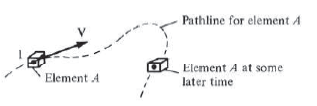
\includegraphics{elementApathline.png}
    \centering
\end{figure}
\noindent
\\Now let time pass a bit and again take a look at a fluid element going through the \emph{same point in space}. This time we are looking at a different fluid element, say B. Let us do the same thing: observe its motion and take several photographs, tracing the path it follows through space. It might look like this (diagram from Anderson's again): \\ \\

\begin{figure}[h]
    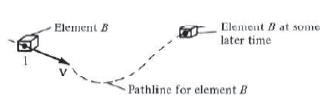
\includegraphics{elementBpathline.png}
    \centering
\end{figure}
\noindent
\\Notice that the paths traced by the two fluid elements are different! This makes sense: the velocity field is a function of time, so the two separate fluid elements that go through the same point at different times will travel through completely different velocity fields. \\ \\
\noindent
The lines we just traced are called \emph{pathlines}, and they are the paths traced by fluid elements that go through the same point in space. Note how \emph{pathlines of different fluid elements are different from each other in unsteady flow}.\\ \\
\noindent
Let's instead do another experiment. Instead of taking several pictures of the fluid element, let us take only one picture. Imagine also that we are an omnipotent being such that we know the flow variables everywhere always. For that one instant we can trace a line that is tangent to the velocity field everywhere. \emph{This line is the streamline}. The key difference here is that the streamline is a snapshot - we are only looking at one picture! If we take another picture after the fluid element moves a bit, then the velocity field will have changed completely (it is a function of time!) so the streamline will have changed too. Just as Anderson puts it:

\begin{quote}
    \emph{You can visualize a pathline as a time-exposure photograph of a given fluid element, whereas a streamline pattern is like a single frame of a motion picture of the flow. In an unsteady flow, the streamline pattern changes; hence, each “frame” of the motion picture is different.} - Anderson's Fundamentals of Aerodynamics, 6$^{th}$ edition
\end{quote}
\noindent
Let us instead consider the case of \emph{steady flow}. Repeating the two experiments, we will notice that:

\begin{enumerate}
    \item The pathlines for two different fluid elements going through the same point are the same and;
    \item The pathlines coincide with the streamline
\end{enumerate}
This is intuitive: the velocity field is now independent of time, so two fluid elements going through the same point at different times will follow the same path! Also, if we take a snapshot at any time of the flow, the velocity field is the same, so the streamlines don't change in time and match the pathlines exactly. \\ \\
\noindent
We will later want to plot streamlines for different Potential Flows. It is useful, therefore, to have some quantitative description of these curves - ideally, we would want an equation for them. Let us find just that.

\subsection{Quantitative Description of Streamlines}
Consider a particle moving through space in steady flow. The streamline is represented below: \\ \\

\begin{figure}[h]
    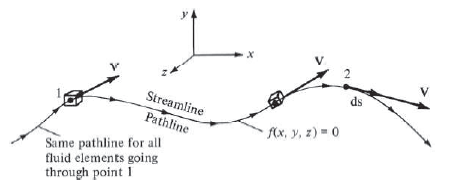
\includegraphics{streamline.png}
    \centering
\end{figure}
\noindent
\\By definition, the streamline is tangent to the velocity vector everywhere. Let $\vec{\bm{ds}}$ be the infinitesimal displacement of the fluid element, and $\vec{\bm{u}}$ be the velocity vector at that point in space. Let's use the following identity of cross products: if $\vec{\bm{A}}$ and $\vec{\bm{B}}$ are parallel, then $\vec{\bm{A}} \times \vec{\bm{B}} = 0$. For the streamline, this implies that:

\begin{equation*}
    \vec{\bm{u}} \times \vec{\bm{ds}} = 0
\end{equation*}\\
\noindent
Everywhere in the flow-field. The velocity and displacement vectors are:

\begin{equation*}
    \vec{\bm{u}} =  \begin{bmatrix}
        u \\
        v \\
        w \\     
        \end{bmatrix}
\end{equation*}

\begin{equation*}
    \vec{\bm{ds}} =  \begin{bmatrix}
        dx \\
        dy \\
        dz \\     
        \end{bmatrix}
\end{equation*} \\ 
\noindent
And so their cross product is:

\begin{equation*}
    \begin{bmatrix}
        u \\
        v \\
        w \\     
    \end{bmatrix} \times \begin{bmatrix}
            dx \\
            dy \\
            dz \\     
    \end{bmatrix} = \begin{vmatrix}
        \hat{i} & \hat{j} & \hat{k} \\
        u & v & w \\
        dx & dy & dz
    \end{vmatrix} = \begin{bmatrix}
        v\,dz - w\,dy \\
        w\,dx - u\,dz \\
        u\,dy - v\,dx \\     
        \end{bmatrix} = 0
\end{equation*} \\ 
\noindent
Therefore, each element must be zero, and we have:

\begin{equation*}
    \begin{matrix}
        v\,dz - w\,dy = 0\\
        w\,dx - u\,dz = 0\\
        u\,dy - v\,dx = 0\\ 
    \end{matrix}
\end{equation*}\\
\noindent
The expressions above are differential equations for the streamline, and can be integrated in space to find the equation for the streamline. Remarkably simple! \\ \\
\noindent
We are particularly interested in 2D flow in the xy plane. In that case, the differential equation for a streamline is simply:

\begin{equation*}
    \frac{dy}{dx} = \frac{v}{u}
\end{equation*} \\
\noindent
Which can also be written as:

\begin{equation*}
    v\,dx - u\,dy = 0
\end{equation*}
\pagebreak

\section{Vorticity and Circulation}
Two additional tools are introduced below, which are the vorticity and circulation. The vorticity is closely related to how rotational a flow is - or the angular velocity that a fluid element develops as it moves along a flow-field. Circulation is closely related to the generation of lift, as will later be revealed.

\subsection{Angular Velocity and Vorticity}
Consider a fluid element moving through a streamline and let us ignore the presence or absence of shear stresses, that is, let us not look at the forces (dynamics) but solely at the motion (kinematics) of the parcel. \\ \\
\noindent
The fluid element's motion is a combination of translation (changing x, y, and z location), rotation, and deformation. The figure below illustrates what that might look like: \\ \\ 

\begin{figure}[h]
    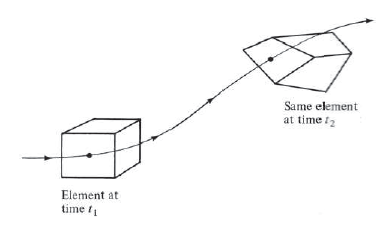
\includegraphics{elementrottrans.png}
    \centering
\end{figure}
\noindent
It is fruitful for us to try to quantitatively describe the rotation of the fluid element. It can be shown that the angular velocity $\vec{\bm{\zeta}}$ of a fluid element in a velocity field $\vec{\bm{u}} = \vec{\bm{u}}(x, y, z)$ is:

\begin{equation*}
    \vec{\bm{\zeta}} = \frac{1}{2}\left[\left(\frac{\partial w}{\partial y} - \frac{\partial v}{\partial z}\right)\hat{\bm{i}} + \left(\frac{\partial u}{\partial z} - \frac{\partial w}{\partial x}\right)\hat{\bm{j}}+\left(\frac{\partial v}{\partial x} - \frac{\partial u}{\partial y}\right)\hat{\bm{k}}\right]
\end{equation*}\\
\noindent
Notice the similarity to a cross product here. In fact, the quantity $2\vec{\bm{\zeta}}$ appears so frequently that it is useful to define a new quantity, the \emph{vorticity} $\vec{\bm{\omega}}$:

\begin{equation*}
    \vec{\bm{\omega}} = 2\vec{\bm{\zeta}}
\end{equation*} \\ 
\noindent
And note from the expression above that:

\begin{equation*}
    \vec{\bm{\omega}} = \nabla \times \vec{\bm{u}}
\end{equation*}\\
\noindent
That is, \emph{the vorticity is simply the curl of the velocity} and is closely related to the angular velocity developed by a fluid element. We can now speak of the rotationality of the flow, that is, we have created two categories of flow:

\begin{enumerate}
    \item Rotational Flow: $\vec{\bm{\omega}} \neq 0$
    \item Irrotational Flow: $\vec{\bm{\omega}} = 0$
\end{enumerate}
\noindent
And the physical meaning being that in rotational flow, the fluid elements does not maintain its orientation along a streamline, but in irrotational flow it does. Also, it can be shown that \emph{all viscous flow is rotational}, which is somewhat intuitive due to the presence of shear stresses creating moment couples in the fluid element. \\ \\
\noindent
Lastly, note that in 2D flow in the xy plane, the vorticity is simply:

\begin{equation*}
    \vec{\bm{\omega}} = \left( \frac{\partial v}{\partial x} - \frac{\partial u}{\partial y} \right) \hat{\bm{k}}
\end{equation*}

\subsection{Circulation}
Consider a velocity field $\vec{\bm{u}}$ and an arbitrary closed curve $C$. The circulation $\Gamma$ is defined as the negative of the line integral around the closed curve. We write:

\begin{equation*}
    \Gamma = - \oint_C\vec{\bm{u}}\cdot\vec{\bm{dr}}
\end{equation*} \\
\noindent
The significance of circulation will become more clear later on, but it is intrinsically related to lift. In fact, two scientists independently used circulation to discover what is known as the Kutta-Joukowski theorem:

\begin{equation*}
    L' = \rho_\infty u_\infty \Gamma
\end{equation*}\\
\noindent
Where $L'$ is the lift per unit span. This is a remarkable result and has very useful implications. For instance, given a closed curve $C$ around an airfoil, the airfoil will generate lift if the line integral is non-zero (finite) - that is, if the circulation is finite. \\ \\
\noindent
We can make use of a theorem of vector calculus to rewrite circulation in terms of vorticity. Recall Stokes' Theorem \eqref{stokesTheorem} reproduced below:

\begin{equation*}
    \oint_C \vec{\bm{A}} \cdot \vec{\bm{dr}} = \iint_S (\nabla \times \vec{\bm{A}}) \cdot \vec{\bm{dS}}
\end{equation*} \\
\noindent
So we can rewrite the circulation in terms of vorticity:

\begin{equation*}
    \Gamma = -\iint_S (\nabla \times \vec{\bm{u}}) \cdot \vec{\bm{dS}} = -\iint_S \vec{\bm{\omega}} \cdot \vec{\bm{dS}}
\end{equation*} \\
\noindent
A powerful result. Lastly, we can write the equation above in differntial form by taking an infinitesimally small control area. We then have:

\begin{equation*}
    d\Gamma = -\vec{\bm{\omega}}\cdot\vec{\bm{dS}} = -\vec{\bm{\omega}}\cdot\hat{\bm{n}}\,dS
\end{equation*} \\
We then arrive at the following result:

\begin{equation*}
    \vec{\bm{\omega}}\cdot\hat{\bm{n}} = -\frac{d\Gamma}{dS}
\end{equation*} \\
\noindent
So the normal component of vorticity is the circulation per unit area. This will come in handy later.
\pagebreak

\section{Stream Function and Velocity Potential}
Lastly, we are ready to introduce the last tools we need to explore Potential Flow and its solutions. These are the streamfunctions and velocity potentials. These are useful tools in working out the kinematics of the flow, and are closely related to the conservation laws and assumptions of Potential Flow.

\subsection{Stream Function}
Stream Functions are closely related to streamlines as shown below. Recall the equation of a streamline for 2D flow in the xy plane, the simplifying case that we will consider from now on:

\begin{equation*}
    \frac{dy}{dx} = \frac{v}{u}
\end{equation*} \\
\noindent
This is a differential equation. Integrating it will yield some function of $x$ and $y$ plus some constant, such that:

\begin{equation*}
    f(x,y) = c
\end{equation*} \\
\noindent
This function is none other than the function defining a streamline. We will now call it the stream function and denote it by $\psi$ such that:

\begin{equation*}
    \psi(x,y) = c
\end{equation*} \\
\noindent
Meaning that in order to get the equation of a streamline we must set the stream function to a constant. In other words, \emph{lines of constant stream function are streamlines}.\\ \\
\noindent
What is, then, the stream function equal to? The derivation of stream functions is beyond the scope of this text, but the results below can be shown by analyzing streamlines and applying conservation of mass along them. Keep this assumption in mind - that mass is conserved. It can thus be shown that: \\

\begin{equation}\label{streamfunctions}
    \begin{matrix}
        u = \frac{\partial \psi}{\partial y} \\ \\
        v = -\frac{\partial \psi}{\partial x}
    \end{matrix}
\end{equation}\\ \\
\noindent
So the stream function can be found by integrating the above differential equations if the velocity field is known. This is not always the case but, in Potential Flow, we will investigate a few key fundamental flows whose velocity fields are known and, by supperposing several of them, we will obtain more complex flows. This will become more clear later.\\ \\
\noindent
Some of these key fundamental flows are more conveniently expressed not in terms of $u$ and $v$ (cartesian coordinates) but rather in terms of radial and angular components of velocity, that is, $u_r$ and $u_\theta$. It is therefore useful to introduce these velocities in terms of the stream functions, which is very similar to the above but adjusted for the transformation (Jacobian). We have:

\begin{equation}\label{streamfunctionspolar}
    \begin{matrix}
        u_r = \frac{1}{r}\frac{\partial\psi}{\partial\theta} \\ \\
        u_\theta = -\frac{\partial\psi}{\partial r}
    \end{matrix}
\end{equation}\\ \\
\noindent
Are the radial and angular velocities in terms of the stream function in polar coordinates.\\ \\
\noindent
Lastly, some further insight can be obtained from the derivation of the stream function (which the reader is encouraged to seek out.) It can be shown that the difference between two adjacent constant stream functions, that is, between two streamlines given by:

\begin{equation*}
    \Delta\psi = c_2 - c_1
\end{equation*}\\ 
\noindent
Is numerically the \emph{volume flow per unit depth} between the two streamlines. In SI, it has units of cubic meters per second per meter perpendicular into the page, or simply $m^2/s$.\\ \\
\noindent
It is also important to note that (\ref{streamfunctions}) and (\ref{streamfunctionspolar}) define the stream functions for incompressible flow. In the case of compressible flow, we would have $\rho u = \partial \bar{\psi} / \partial y$ and $\rho v = -\partial \bar{\psi} / \partial x$ where the "bar" is used to distinguish between the compressible and incompressible stream functions, since $\psi = \bar{\psi} / \rho$

\subsection{Stream Function and Conservation of Mass}
This insight is of particular importance so it deserves its own subsection, despite it being somewhat short. \\ \\
\noindent
Recall the differential form of conservation of mass (\ref{continuity}):

\begin{equation*}
    \frac{D\rho}{Dt} + \rho\nabla \cdot \vec{\bm{u}} = 0
\end{equation*}\\
\noindent
For incompressible flow, that is, constant density, it is easy ton see that the above is reduced to:

\begin{equation*}
    \nabla \cdot \vec{\bm{u}} = 0
\end{equation*}\\
\noindent
In 2D flow in the xy plane, the divergence of the velocity is simply

\begin{equation*}
    \nabla \cdot \vec{\bm{u}} = \frac{\partial u}{\partial x} + \frac{\partial v}{\partial y}
\end{equation*}\\ 
\noindent
Let's write this in terms of the stream function that we just found. Subtituting $u = \frac{\partial \psi}{\partial y}$ and $v = -\frac{\partial \psi}{\partial x}$ gives:

\begin{equation*}
    \frac{\partial u}{\partial x} + \frac{\partial v}{\partial y} = \frac{\partial^2\psi}{\partial x \partial y} - \frac{\partial^2\psi}{\partial x \partial y} = 0
\end{equation*} \\ 
\noindent
Which satisfies the continuity equation! This is an important result: \emph{the stream function, by definition, satisfies conservation of mass.} In other words, if a stream function exists everywhere for a velocity field $\vec{\bm{u}}$ then the velocity field satisfies conservation of mass everywhere. The converse is also true: if a velocity field satisfies conservation of mass everywhere, then there must exist a stream function $\psi(x,y)$.

\subsection{Velocity Potential}
Just as the stream function automatically satisfies the continuity condition, we can try to satisfy other conditions to find equations that govern flow under certain assumptions. Let us do this for the case of vorticity.\\ \\
\noindent
Recall vorticity is simply the curl of velocity, $\vec{\bm{\omega}} = \nabla \times \vec{\bm{u}}$. Therefore, for irrotational flow, the following must be true:

\begin{equation*}
    \nabla \times \vec{\bm{u}} = 0
\end{equation*}\\
\noindent
Let us now make use of the following useful identity in vector algebra: the curl of the gradient of a scalar is zero. That is, for a scalar-valued function $\phi$ it is true that:

\begin{equation*}
    \nabla \times (\nabla\phi) = 0
\end{equation*}\\
\noindent
This leads to the following useful conclusion: \emph{if the velocity} $\vec{\bm{u}}$ \emph{can be written in terms of the gradient of a vector-valued function everywhere, then we guarantee that the velocity field is irrotational everywhere!} We therefore define a scalar-valued \emph{velocity potential} $\phi(x,y)$ such that:

\begin{equation}\label{velocitypotential}
    \vec{\bm{u}} = \nabla \phi
\end{equation}\\
\noindent
Whose existence implies irrotationality. The converse is also true: irrotationality implies the existence of a velocity potential $\phi$. We can therefore write:

\begin{equation*}
    \begin{matrix}
        u = \frac{\partial \phi}{\partial x} \\ \\
        v = \frac{\partial \phi}{\partial y} \\ \\
        w = \frac{\partial \phi}{\partial z}
    \end{matrix}
\end{equation*}\\
\noindent
Are the velocity field components in terms of the velocity potential, such that if the velocity components are known the potential can be found by integrating the above differential equations. They can also be written in polar coordinates much like we did for stream functions:

\begin{equation*}
    \begin{matrix}
        u_r = \frac{\partial \phi}{\partial r} \\ \\
        u_\theta = \frac{1}{r}\frac{\partial \phi}{\partial \theta}
    \end{matrix}
\end{equation*}

\subsection{Relation between $\bm{\psi(x,y)}$ and $\bm{\phi(x,y)}$}
The stream function and velocity potential are intrinsically related. However, it is important to point out a few key distinctions between the two:

\begin{enumerate}
    \item We obtain $\vec{\bm{u}}$ by differentiating the velocity potential $\phi$ in the same direction as the velocity. However, we must differentiate $\psi$ in the direction normal to the velocity to obtain $\vec{\bm{u}}$;
    \item The stream function is defined for both rotational and irrotational flows. However, \emph{the velocity potential is defined for irrotational flow only};
    \item The velocity potential applies to 3D flow, whereas the stream function is defined only for 2D flow.
\end{enumerate}
\noindent
Despite these differences, there is a key connection between stream functions and velocity potentials. Consider 2D, irrotational (there exists a potential) and incompressible flow. The stream lines are lines of constant $\psi$, which implies that the total differential $d\psi = 0$. But the total differential is:

\begin{equation*}
    d\psi = \frac{\partial \psi}{\partial x}dx + \frac{\partial \psi}{\partial y}dy = 0
\end{equation*}\\
\noindent
Substituting $\partial \psi / \partial x$ and $\partial \psi / \partial y$:

\begin{equation*}
    -v\,dx + u\,dy = 0
\end{equation*}\\
\noindent
Rearranging to find $dy/dx$, that is, the slope of the line of constant stream function yields:

\begin{equation*}
    \left( \frac{dy}{dx} \right)_{\psi = \textnormal{const}} = \frac{v}{u}
\end{equation*}\\
\noindent
Which should look familiar - this is the differential equation for a streamline which we obtained by setting $\psi$ to a constant, as expected.\\ \\
\noindent
Let us now do the same for a line of constant potential, $d\phi = 0$. This yields an interesting result. Expanding the differential:

\begin{equation*}
    d\phi = \frac{\partial \phi}{\partial x}dx + \frac{\partial \phi}{\partial y}dy = 0
\end{equation*} \\ 
\noindent
Substituting the velocity potential derivatives:

\begin{equation*}
    u\,dx + v\,dy = 0
\end{equation*}\\
\noindent
Finally, solving for $dy/dx$ gives:

\begin{equation*}
    \left( \frac{dy}{dx} \right)_{\phi = \textnormal{const}}=-\frac{u}{v}
\end{equation*}\\
Which gives the fascinating fact that:

\begin{equation*}
    \left( \frac{dy}{dx} \right)_{\phi = \textnormal{const}} = -\frac{1}{\left( dy/dx \right)_{\psi=\textnormal{const}}}
\end{equation*}\\
\noindent
In other words, \emph{streamlines ($\psi = \textnormal{const}$) and equipotential lines ($\phi = \textnormal{const}$) are mutually perpendicular!} Which is quite insightful.
\pagebreak

\section{Potential Flow}
We are now ready to explore Potential Flow and its solutions.

\end{document}